% ---------------------------------------------------------------------------
% VT analysis report — LaTeX template
%
% Rendered by analysis.py with Jinja2. Values are inserted with VAR placeholders
% and logic with BLOCK statements. Edit the layout and wording freely; keep the
% placeholders. Figures are vector PDFs in report/figures/.
% ---------------------------------------------------------------------------
\documentclass[11pt,a4paper]{article}

\usepackage[T1]{fontenc}
\usepackage[utf8]{inputenc}
\usepackage{mathptmx}
\usepackage[scaled=0.9]{helvet}
\usepackage{courier}
\usepackage[a4paper,margin=2.4cm,top=2.3cm,bottom=2.6cm]{geometry}
\usepackage{microtype}
\usepackage{graphicx}
\usepackage{booktabs}
\usepackage{tabularx}
\usepackage{array}
\usepackage[table]{xcolor}
\usepackage{caption}
\usepackage{enumitem}
\usepackage{titlesec}
\usepackage{fancyhdr}
\usepackage{amsmath}
\usepackage{float}
\usepackage[round]{natbib}
\usepackage{needspace}
\usepackage[hidelinks]{hyperref}

\definecolor{ink}{HTML}{121211}
\definecolor{muted}{HTML}{6E6D68}
\definecolor{accent}{HTML}{1F5FAD}
\definecolor{rule}{HTML}{C9C8C0}

\graphicspath{{figures/}}
\setlength{\parindent}{0pt}
\setlength{\parskip}{0.55em}
\renewcommand{\arraystretch}{1.18}
\setlength{\aboverulesep}{0.25ex}
\setlength{\belowrulesep}{0.4ex}

\titleformat{\section}{\sffamily\Large\bfseries\color{ink}}{\thesection}{0.7em}{}
\titleformat{\subsection}{\sffamily\large\bfseries\color{ink}}{\thesubsection}{0.6em}{}
\titlespacing*{\section}{0pt}{1.6em}{0.6em}
\titlespacing*{\subsection}{0pt}{1.2em}{0.35em}
\newcommand{\keep}[1]{\Needspace{#1\baselineskip}}

\captionsetup{font=small,labelfont={bf,sf},labelsep=period,justification=raggedright,singlelinecheck=false,skip=4pt}
\captionsetup[table]{position=top}

\newcommand{\note}[1]{{\footnotesize\color{muted}#1\par}}
\newcolumntype{R}{>{\raggedleft\arraybackslash}X}
\newcolumntype{L}{>{\raggedright\arraybackslash}X}

\pagestyle{fancy}
\fancyhf{}
\renewcommand{\headrulewidth}{0pt}
\fancyfoot[L]{\footnotesize\color{muted}\sffamily Vanguard Total World Stock ETF (VT) --- Price analysis since inception}
\fancyfoot[R]{\footnotesize\color{muted}\sffamily \thepage}

\hypersetup{pdftitle={VT -- Price analysis since inception}, pdfauthor={Cédric Masset}}

\begin{document}

% ---------------------------------------------------------------- Title
\thispagestyle{fancy}
{\sffamily
{\footnotesize\color{muted}\MakeUppercase{Market data report} \textperiodcentered{} 30 October 2026}\par\vspace{0.6em}
{\fontsize{22}{26}\selectfont\bfseries\color{ink} Vanguard Total World Stock ETF (VT)\par}\vspace{0.3em}
{\large\color{muted} Price analysis since inception, 26 Jun 2008 -- 30 Oct 2026\par}\vspace{0.2em}
{\small\color{muted} Cédric Masset \textperiodcentered{} 4,616 trading days \textperiodcentered{} Yahoo Finance data, validated against Vanguard\par}
}
\vspace{0.4em}

\section*{Summary}

\begin{table}[H]
\footnotesize
\begin{tabularx}{\linewidth}{L r}
\toprule
\textbf{Metric} & \textbf{Value} \\
\midrule
Price at inception $\rightarrow$ latest price & USD 49.58 $\rightarrow$ 155.33 \\
Cumulative return (price / total return) & 213\% / 360\% \\
Annualised return (price / total return) & 6.4\% / 8.7\% \\
Annualised total return in CHF & 7.4\% \\
Annualised volatility (monthly returns; daily $\times\sqrt{252}$ in brackets) & 16.5\% (20.4\%) \\
Sharpe ratio, 95\% confidence interval (average risk-free rate 1.4\%) & 0.50 [0.02, 0.99] \\
Sortino ratio & 0.73 \\
Maximum drawdown (total return) & $-$50.3\% (trough on 09 Mar 2009) \\
Calmar ratio & 0.17 \\
Probability of loss over 1 / 5 / 10 years: historical windows & 22\% / 0\% / 0\% \\
Probability of loss over 1 / 5 / 10 years: block bootstrap & 24\% / 10\% / 4\% \\
\bottomrule
\end{tabularx}
\end{table}

\subsection*{Key findings}
\begin{itemize}[leftmargin=1.2em,itemsep=0.3em,topsep=0.2em]
  \item Over 18.3 years, VT returned 8.7\% a year with dividends reinvested, of which roughly 2.2\% a year came from dividends. These figures match Vanguard's published market-price returns to within 0.01 percentage point.
  \item Measured on monthly returns, annualised volatility is 16.5\%; scaling daily volatility by $\sqrt{252}$ gives 20.4\% because daily returns are negatively autocorrelated. The maximum drawdown was $-$50\% during the global financial crisis.
  \item The Sharpe ratio of 0.50 has a 95\% confidence interval of [0.02, 0.99]: eighteen years of data are barely enough to distinguish it from zero.
  \item Daily returns have fat tails (kurtosis 16.1) and strongly persistent volatility (GARCH persistence 0.993, half-life of about 96 trading days). A GARCH(1,1)-$t$ model forecasts the 5\% Value at Risk well out of sample; rolling historical and normal VaR do not, because their breaches cluster.
  \item After correcting for multiple testing, the only departure from a random walk is a small negative autocorrelation of daily returns ($-$0.105); it vanishes at weekly and monthly frequencies. No calendar effect is significant, and a 200-day moving-average rule underperformed buy and hold.
  \item For a Swiss franc investor, the weaker dollar cut the annualised return by 1.3\% (7.4\% in CHF), before taxes.
\end{itemize}

\clearpage
% ---------------------------------------------------------------- 1
\section{Return and risk}

\begin{figure}[H]
\centering
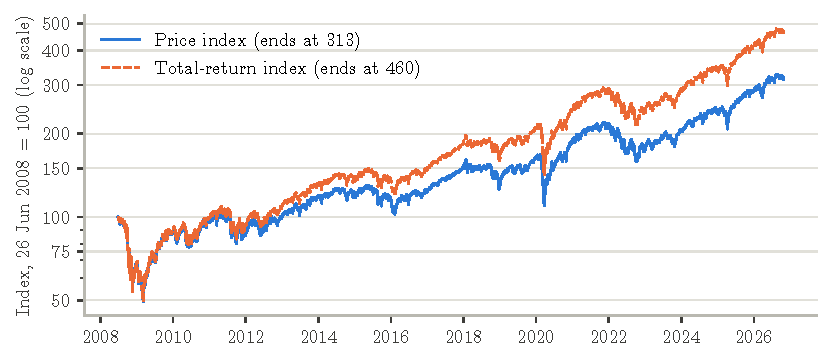
\includegraphics[width=\linewidth]{price.pdf}
\caption{Closing price and total return (dividends reinvested), USD, log scale. Equal slopes represent equal percentage returns; the widening gap reflects reinvested dividends.}
\end{figure}

\keep{16}\subsection{Calendar-year returns}
\begin{figure}[H]
\centering
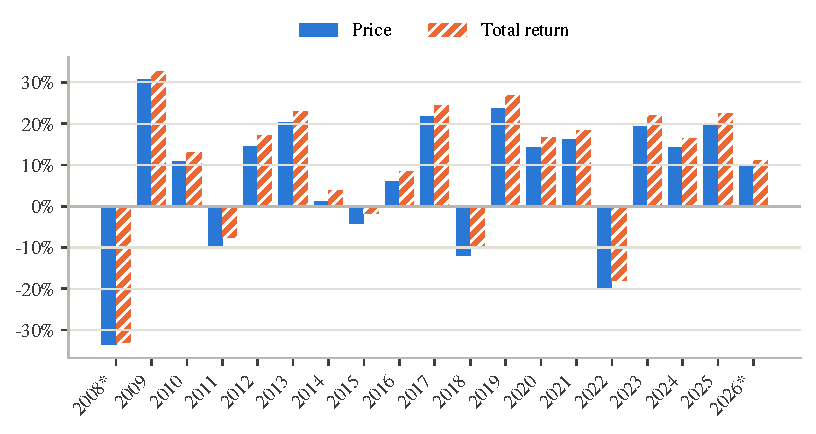
\includegraphics[width=\linewidth]{annual.pdf}
\caption{Calendar-year returns, price and total return. * Partial years.}
\end{figure}
\note{* Partial years: 2008 (from inception) and 2026 (up to 30 Oct 2026). Of the 17 full years, the best was 2009 (+32.7\%) and the worst 2022 ($-$18.0\%); 4 years were negative.}

\keep{16}\subsection{Volatility}
\begin{figure}[H]
\centering
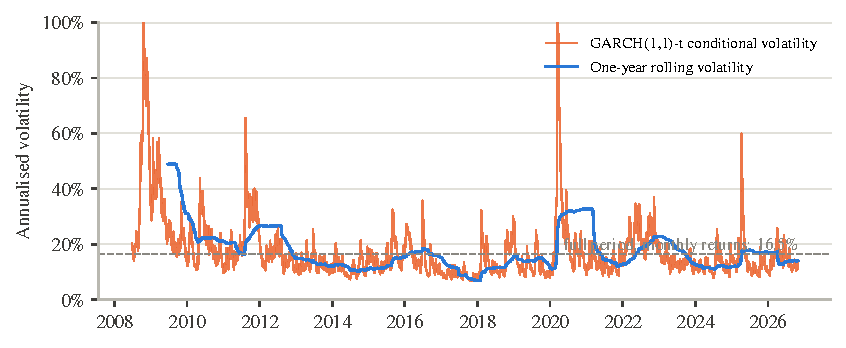
\includegraphics[width=\linewidth]{volatility.pdf}
\caption{Annualised volatility: one-year rolling window of daily returns and GARCH(1,1)-$t$ conditional volatility (daily, $\times\sqrt{252}$).}
\end{figure}

\begin{table}[H]
\small
\caption{Annualised volatility by sampling frequency (non-overlapping total returns).}
\begin{tabularx}{\linewidth}{L r r}
\toprule
\textbf{Frequency} & \textbf{Observations} & \textbf{Annualised volatility} \\
\midrule
Daily & 4,615 & 20.4\% \\
Weekly & 957 & 18.3\% \\
Monthly & 220 & 16.6\% \\
Quarterly & 74 & 17.8\% \\
\bottomrule
\end{tabularx}
\end{table}
Volatility varies sharply across regimes: the one-year rolling estimate ranges from 7\% (year ending 14 Dec 2017) to 49\% (year ending 23 Jul 2009), and the GARCH conditional volatility peaks at 111\% on 17 Mar 2020.

The annualised level also depends on the sampling frequency. Scaling a $k$-period standard deviation by $\sqrt{k}$ is valid only if returns are serially uncorrelated. Daily returns are negatively autocorrelated (Section~3), so daily data annualised with $\sqrt{252}$ give 20.4\%, whereas monthly data give 16.6\%. The ratio of the two variances, 0.66, is of the same order as the variance ratio estimated in Section~3 at a 20-day horizon (0.76), given the sampling error of only 220 monthly observations. This report therefore uses monthly returns for annualised volatility and for the Sharpe and Sortino ratios.

\keep{16}\subsection{Drawdowns}
\begin{figure}[H]
\centering
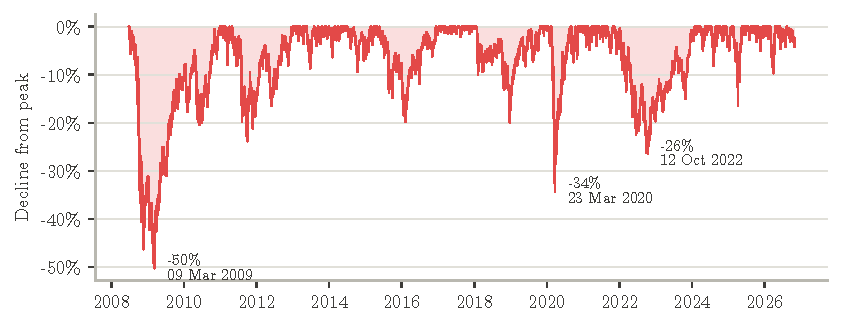
\includegraphics[width=\linewidth]{drawdown.pdf}
\caption{Decline of the total-return index from its previous peak.}
\end{figure}

\begin{table}[H]
\small
\caption{Five largest drawdowns (total return).}
\begin{tabularx}{\linewidth}{l l l R R R}
\toprule
\textbf{Peak} & \textbf{Trough} & \textbf{Recovery} & \textbf{Drawdown} & \textbf{Decline (days)} & \textbf{Recovery (days)} \\
\midrule
26 Jun 2008 & 09 Mar 2009 & 29 Dec 2010 & $-$50.3\% & 175 & 457 \\
12 Feb 2020 & 23 Mar 2020 & 24 Aug 2020 & $-$34.2\% & 27 & 107 \\
08 Nov 2021 & 12 Oct 2022 & 29 Jan 2024 & $-$26.4\% & 233 & 324 \\
29 Apr 2011 & 03 Oct 2011 & 02 Jan 2013 & $-$23.8\% & 108 & 313 \\
26 Jan 2018 & 24 Dec 2018 & 28 Oct 2019 & $-$20.0\% & 229 & 212 \\
\bottomrule
\end{tabularx}
\end{table}
\note{Lengths in trading days. Because VT was launched during the global financial crisis, the first peak is the launch date itself.}

\keep{16}\subsection{Risk-adjusted performance by sub-period}
\begin{table}[H]
\small
\caption{Return and risk by sub-period (total return; volatility and ratios from monthly returns).}
\begin{tabularx}{\linewidth}{L r r r c r r}
\toprule
\textbf{Period} & \textbf{Ann.\ return} & \textbf{Volatility} & \textbf{Sharpe} & \textbf{95\% CI} & \textbf{Sortino} & \textbf{Max.\ DD} \\
\midrule
2008--2012 & 1.9\% & 22.8\% & 0.19 & [$-$0.74, 1.12] & 0.26 & $-$50.3\% \\
2013--2017 & 11.1\% & 10.0\% & 1.07 & [0.15, 1.99] & 1.88 & $-$19.8\% \\
2018--2022 & 5.3\% & 17.9\% & 0.31 & [$-$0.59, 1.20] & 0.44 & $-$34.2\% \\
2023--2026 & 18.8\% & 12.2\% & 1.11 & [0.10, 2.13] & 2.10 & $-$16.5\% \\
\midrule{}Full period & 8.7\% & 16.5\% & 0.50 & [0.02, 0.99] & 0.73 & $-$50.3\% \\
\bottomrule
\end{tabularx}
\end{table}
\note{Excess returns over the 13-week US T-bill (\texttt{\^{}IRX}). Sharpe: mean excess return divided by its volatility. Sortino: mean excess return divided by the downside deviation of excess returns. Confidence intervals for the Sharpe ratio use the standard error of \citet{mertens2002} and \citet{opdyke2007}, which accounts for skewness and kurtosis.}

The confidence intervals are wide: with about five years of monthly data per sub-period, all four sub-period intervals contain the full-period Sharpe ratio, and two contain zero. Differences between sub-periods should be read as descriptive rather than as evidence of a change in the fund's risk-return profile.

% ---------------------------------------------------------------- 2
\keep{24}
\section{Distribution, volatility dynamics and Value at Risk}

\begin{figure}[H]
\centering
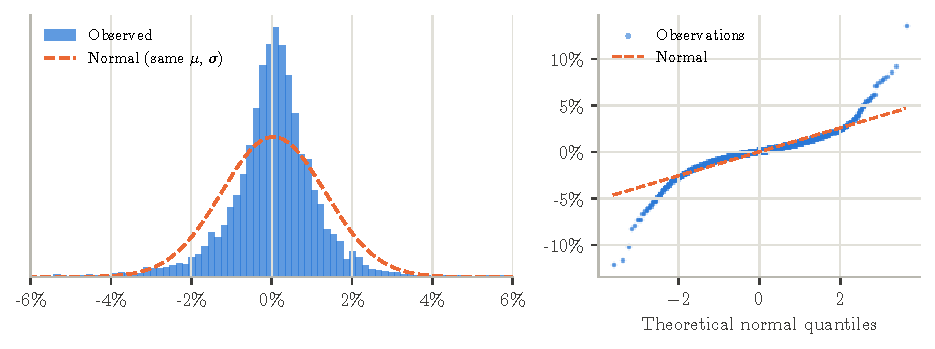
\includegraphics[width=\linewidth]{distribution.pdf}
\caption{Daily total returns: histogram against a normal density with the same mean and variance (left), and normal Q--Q plot (right).}
\end{figure}

\begin{table}[H]
\small
\caption{Descriptive statistics of daily returns.}
\begin{tabularx}{\linewidth}{L r r}
\toprule
\textbf{Statistic} & \textbf{Value} & \textbf{Normal benchmark} \\
\midrule
Mean / standard deviation & 0.041\% / 1.29\% & -- \\
Skewness & $-$0.30 & 0 \\
Kurtosis & 16.08 & 3 \\
Jarque--Bera statistic & 32,989 ($p$ $<$ 0.001) & -- \\
Days beyond $\pm 4$ standard deviations & 47 & 0.29 expected \\
Worst day & $-$12.1\% (15 Oct 2008) & -- \\
Best day & +13.5\% (13 Oct 2008) & -- \\
\bottomrule
\end{tabularx}
\end{table}
The tails are far fatter than those of a normal distribution: 47 days moved by more than four standard deviations, whereas a normal distribution would predict 0.3 over the period. The negative skewness means that large declines are more pronounced than large gains. Part of this excess kurtosis reflects time-varying volatility: returns are closer to normal once scaled by their conditional volatility, as the GARCH estimates below show.

\keep{16}\subsection{Volatility clustering and GARCH estimates}
\begin{figure}[H]
\centering
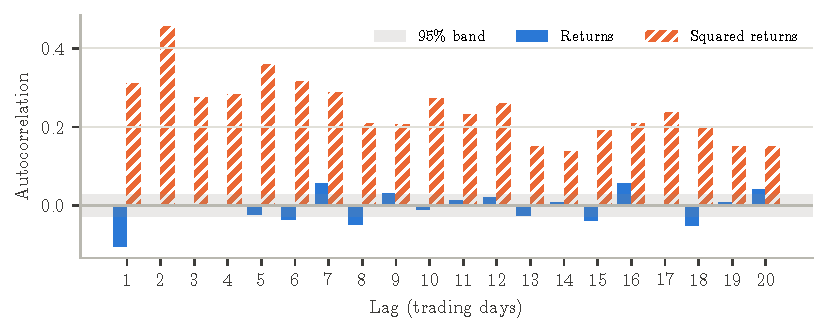
\includegraphics[width=\linewidth]{acf.pdf}
\caption{Autocorrelation of daily log returns and squared log returns, lags 1 to 20, with the 95\% band under independence.}
\end{figure}
Returns show little autocorrelation beyond the first lag (Ljung--Box with 10 lags: $Q = 89.7$). Squared returns, by contrast, are strongly and persistently autocorrelated ($Q = 4,305$, $p < 0.001$): a large move tends to be followed by further large moves of either sign.

\begin{table}[H]
\small
\caption{GARCH(1,1) with standardised Student-$t$ innovations, maximum-likelihood estimates (full sample).}
\begin{tabularx}{\linewidth}{L r r}
\toprule
\textbf{Parameter} & \textbf{Estimate} & \textbf{Standard error} \\
\midrule
$\mu$ (\% per day) & 0.0846 & 0.0110 \\
$\omega$ & 0.0199 & 0.0041 \\
$\alpha$ & 0.1345 & 0.0134 \\
$\beta$ & 0.8583 & 0.0125 \\
$\nu$ (degrees of freedom) & 6.1515 & 0.5503 \\
\bottomrule
\end{tabularx}
\end{table}
\note{Standard errors from the inverse of the numerical Hessian of the log-likelihood.}

The model $\sigma_t^2 = \omega + \alpha\,\varepsilon_{t-1}^2 + \beta\,\sigma_{t-1}^2$ with standardised Student-$t$ innovations is estimated by maximum likelihood on daily log returns in percent \citep{bollerslev1986}. Persistence $\alpha + \beta = 0.993$ implies that a volatility shock loses half its effect after about 96 trading days. The estimated $\nu = 6.2$ confirms that, even after accounting for volatility clustering, daily shocks have fatter tails than the normal distribution. The implied long-run volatility, 26.4\%, uses daily scaling and is therefore comparable with the daily-scaled figure in Section~1.

\keep{16}\subsection{Value at Risk: out-of-sample backtest}
\begin{figure}[H]
\centering
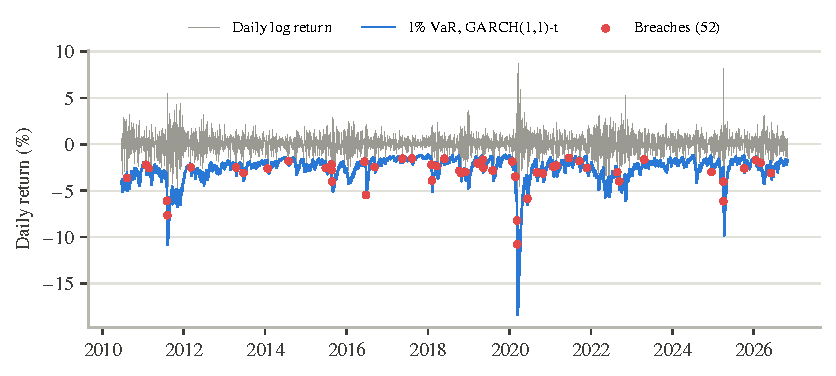
\includegraphics[width=\linewidth]{var_backtest.pdf}
\caption{Daily returns and one-day 1\% VaR forecast by the GARCH(1,1)-$t$ model; red dots mark breaches.}
\end{figure}

\begin{table}[H]
\small
\caption{Backtest of one-day VaR forecasts (4,115 days from 23 Jun 2010); $p$-values of the coverage tests.}
\begin{tabularx}{\linewidth}{l L r r r r r}
\toprule
\textbf{Level} & \textbf{Method} & \textbf{Breach rate} & \textbf{Breaches / expected} & \textbf{Kupiec} & \textbf{Christoff.} & \textbf{CC} \\
\midrule
5\% & Historical (250 days) & 5.20\% & 214 / 206 & 0.558 & $<$ 0.001 & $<$ 0.001 \\
5\% & Normal (250 days) & 5.22\% & 215 / 206 & 0.511 & $<$ 0.001 & $<$ 0.001 \\
5\% & GARCH(1,1)-t & 5.35\% & 220 / 206 & 0.313 & 0.929 & 0.599 \\
1\% & Historical (250 days) & 1.36\% & 56 / 41 & 0.027 & $<$ 0.001 & $<$ 0.001 \\
1\% & Normal (250 days) & 2.38\% & 98 / 41 & $<$ 0.001 & $<$ 0.001 & $<$ 0.001 \\
1\% & GARCH(1,1)-t & 1.26\% & 52 / 41 & 0.102 & 0.004 & 0.004 \\
\bottomrule
\end{tabularx}
\end{table}
\note{One-day VaR on daily log returns, forecasts from 23 Jun 2010 to 30 Oct 2026 (4,115 days), each using only information available the day before. Historical and normal VaR use a 250-day rolling window. GARCH parameters are re-estimated at the start of each calendar year on all prior data, and the conditional variance is updated daily. The GARCH forecasts use a zero conditional mean, standard at a one-day horizon; with the maximum-likelihood location estimate instead (0.085\% a day, well above the sample mean of 0.033\% because of negative skewness), the breach rates rise to 6.10\% and 1.46\%. Kupiec: unconditional coverage; Christoffersen: independence; CC: conditional coverage (joint).}

Rolling historical and normal VaR react slowly to changes in volatility. Their breach rates at 5\% are close to the target, but the breaches cluster in turbulent periods, so the independence test of \citet{christoffersen1998} rejects them decisively. At 1\%, both also fail the unconditional coverage test of \citet{kupiec1995}: 1.36\% and 2.38\% of breaches instead of 1\%. The GARCH(1,1)-$t$ forecasts pass both tests at 5\% (breach rate 5.35\%; $p$-values 0.313 and 0.929). At 1\%, their breach rate of 1.26\% is acceptable ($p = 0.102$), but extreme losses still arrive in clusters ($p = 0.004$ for independence). A symmetric $t$ distribution cannot reproduce the negative skewness of large losses; a skewed distribution or an extreme-value model would be the natural next step.

% ---------------------------------------------------------------- 3
\keep{24}
\section{Market efficiency}

\subsection{First-order autocorrelation}
\begin{table}[H]
\small
\caption{First-order autocorrelation of log returns.}
\begin{tabularx}{\linewidth}{L r r r r r r}
\toprule
\textbf{Frequency} & \textbf{Obs.} & \textbf{$\hat\rho_1$} & \textbf{Naive $t$} & \textbf{Robust $z$} & \textbf{$p$-value} & \textbf{Holm $p$} \\
\midrule
Daily & 4,615 & $-$0.105 & $-$7.16 & $-$2.98 & 0.003 & 0.029 \\
Weekly & 957 & $-$0.023 & $-$0.72 & $-$0.34 & 0.734 & 1.000 \\
Monthly & 220 & 0.033 & 0.49 & 0.33 & 0.742 & 1.000 \\
\bottomrule
\end{tabularx}
\end{table}
\note{Naive $t = \hat\rho_1\sqrt{n}$ assumes independent, identically distributed returns. The robust $z$ uses the heteroskedasticity-consistent standard error $\sqrt{\sum e_t^2 e_{t-1}^2}\,/\sum e_t^2$; $p$-values refer to the robust statistic. Holm: adjusted for the 10 tests of this section.}

Daily autocorrelation is negative ($-$0.105): a gain tends to be slightly reversed the following day. The naive $t$-statistic overstates its significance; the heteroskedasticity-robust statistic is $-$2.98, still significant after the Holm correction. The effect is concentrated in crises: excluding 2008--2009 and February to June 2020, the autocorrelation falls to $-$0.044. Plausible explanations, which these data cannot separate, are overreaction on turbulent days and temporary gaps between the ETF's closing price and the value of its foreign holdings, which trade at different hours. Testing the second would require daily net asset values. At weekly and monthly frequencies, no autocorrelation is detectable.

\keep{16}\subsection{Variance ratio test}
Under the random-walk hypothesis, the variance of $q$-period returns is $q$ times the one-period variance, so
\[
VR(q) = \frac{\operatorname{Var}\left(r_t + r_{t-1} + \dots + r_{t-q+1}\right)}{q \,\operatorname{Var}(r_t)} = 1 .
\]
A ratio below 1 signals mean reversion, a ratio above 1 persistence. Following \citet{lo1988}, the statistic $z^*(q)$ is robust to heteroskedasticity, which is essential given the volatility clustering documented above.

\begin{table}[H]
\small
\caption{Lo--MacKinlay variance ratio test on daily log total returns.}
\begin{tabularx}{\linewidth}{l r r r r R}
\toprule
\textbf{Horizon $q$ (days)} & \textbf{$VR(q)$} & \textbf{$z^*(q)$} & \textbf{$p$-value} & \textbf{Holm $p$} & \textbf{Conclusion (Holm)} \\
\midrule
2 & 0.895 & $-$2.97 & 0.003 & 0.029 & mean reversion \\
5 & 0.830 & $-$2.09 & 0.037 & 0.296 & not rejected \\
10 & 0.778 & $-$1.80 & 0.072 & 0.504 & not rejected \\
20 & 0.760 & $-$1.38 & 0.167 & 1.000 & not rejected \\
\bottomrule
\end{tabularx}
\end{table}

\keep{16}\subsection{Calendar effects}
\begin{figure}[H]
\centering
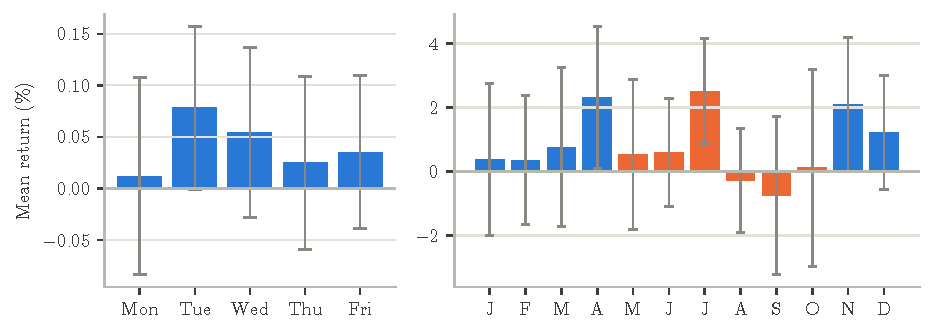
\includegraphics[width=\linewidth]{calendar.pdf}
\caption{Mean daily return by weekday (left) and mean monthly return by calendar month (right), with 95\% confidence intervals. May to October in orange.}
\end{figure}

\begin{table}[H]
\small
\caption{Tests of calendar effects.}
\begin{tabularx}{\linewidth}{L r r r}
\toprule
\textbf{Test} & \textbf{Result} & \textbf{$p$-value} & \textbf{Holm $p$} \\
\midrule
Equal mean returns across weekdays (ANOVA) & $F = 0.38$ & 0.826 & 1.000 \\
January effect: January vs other months (Welch) & 0.38\% vs 0.85\% per month & 0.714 & 1.000 \\
``Sell in May'': Nov--Apr vs May--Oct, per half-year (18 and 18 half-years) & 7.1\% vs 4.7\% & 0.483 & 1.000 \\
\bottomrule
\end{tabularx}
\end{table}
\note{With fewer than twenty observations per calendar month, these tests have little power: the absence of significance does not prove the absence of an effect, only that any effect is too small to detect in eighteen years of data.}

\keep{12}\subsection{Multiple testing}
Section~3 reports 10 hypothesis tests. At the 5\% level, about one false rejection is expected by chance alone, so each $p$-value is also adjusted with the step-down procedure of \citet{holm1979}, which controls the probability of any false rejection. 3 tests are significant before adjustment and 2 after. Both remaining rejections concern the same first-order daily autocorrelation, since $VR(2) \approx 1 + \hat\rho_1$.

\keep{16}\subsection{Moving-average timing rules}
\begin{figure}[H]
\centering
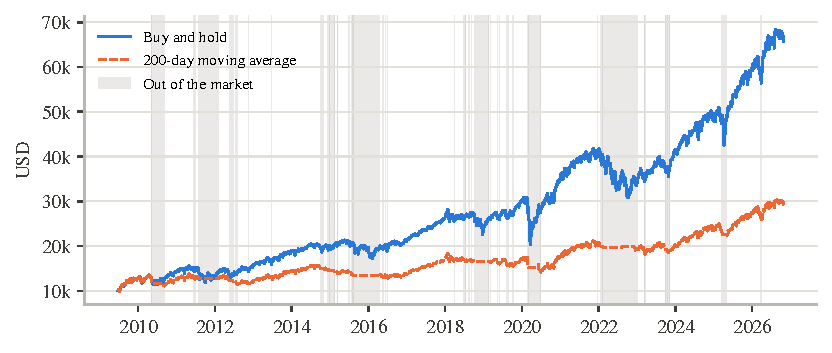
\includegraphics[width=\linewidth]{ma200.pdf}
\caption{Growth of USD 10{,}000 from 24 Jun 2009: buy and hold vs the 200-day moving-average rule. Shaded areas: rule out of the market.}
\end{figure}

\begin{table}[H]
\small
\caption{Buy and hold vs 200-day moving average (Sharpe ratio with 95\% confidence interval).}
\begin{tabularx}{\linewidth}{L r r}
\toprule
 & \textbf{Buy and hold} & \textbf{200-day moving average} \\
\midrule
Annualised return & 11.5\% & 6.4\% \\
Volatility & 14.7\% & 11.2\% \\
Sharpe ratio & 0.71 [0.22, 1.21] & 0.48 [0.00, 0.95] \\
Maximum drawdown & $-$34.2\% & $-$22.5\% \\
Final value of USD 10{,}000 & USD 65,660 & USD 29,231 \\
\bottomrule
\end{tabularx}
\end{table}

\begin{table}[H]
\small
\caption{Sensitivity to the moving-average window (common period).}
\begin{tabularx}{\linewidth}{L r r r r r r}
\toprule
\textbf{Window} & \textbf{Ann.\ return} & \textbf{Volatility} & \textbf{Sharpe} & \textbf{Max.\ DD} & \textbf{Switches} & \textbf{Invested} \\
\midrule
50 days & 3.6\% & 9.6\% & 0.26 & $-$25.9\% & 319 & 68\% \\
100 days & 5.9\% & 10.3\% & 0.47 & $-$25.2\% & 203 & 72\% \\
150 days & 5.6\% & 10.7\% & 0.42 & $-$26.9\% & 176 & 74\% \\
200 days & 6.4\% & 11.2\% & 0.48 & $-$22.5\% & 140 & 77\% \\
250 days & 6.3\% & 11.0\% & 0.48 & $-$23.1\% & 141 & 77\% \\
\midrule{}Buy and hold & 11.5\% & 14.7\% & 0.71 & $-$34.2\% & 0 & 100\% \\
\bottomrule
\end{tabularx}
\end{table}
\note{Rule: invested in VT when the previous day's close is above its moving average, otherwise held in T-bills; switches are executed at that same close and cost 0.10\% each. All windows are compared over the same period, starting 24 Jun 2009, the first day on which a 250-day average is available.}

Every window underperformed buy and hold, by 5.1\% to 7.9\% a year, while reducing the maximum drawdown. For the 200-day rule, a circular block bootstrap (2,000 replications, 63-day blocks) gives a 95\% confidence interval of [0.2\%, 10.3\%] for the annual return gap ($p = 0.051$): the underperformance is borderline significant. The sample starts in mid-2009, after the financial-crisis crash that such rules are designed to avoid, which works against them; a longer index history would be needed for a fair assessment. Late and repeated signals (``whipsaws'') are costly in a market that recovers quickly.

% ---------------------------------------------------------------- 4
\keep{24}
\section{Holding period and investor behaviour}

\subsection{Rolling returns and the probability of loss}
\begin{figure}[H]
\centering
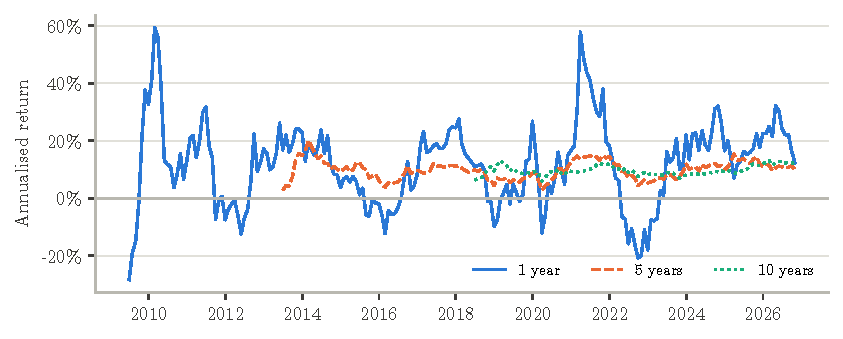
\includegraphics[width=\linewidth]{rolling.pdf}
\caption{Annualised total return over rolling 1-, 5- and 10-year windows, by end of window.}
\end{figure}

\begin{table}[H]
\small
\caption{Rolling returns (overlapping monthly windows, annualised) and bootstrap probability of loss.}
\begin{tabularx}{\linewidth}{l r r r R r r}
\toprule
\textbf{Horizon} & \textbf{Windows} & \textbf{P(loss)} & \textbf{Bootstrap} & \textbf{Worst (window end)} & \textbf{Median} & \textbf{Best} \\
\midrule
1 year & 209 & 22\% & 24\% & $-$28.4\% (Jun 2009) & 13.1\% & 59.3\% \\
5 years & 161 & 0\% & 10\% & 2.8\% (Mar 2020) & 10.1\% & 20.0\% \\
10 years & 101 & 0\% & 4\% & 6.0\% (Mar 2020) & 9.3\% & 13.1\% \\
\bottomrule
\end{tabularx}
\end{table}
Overlapping windows understate the probability of loss at long horizons: the 10-year windows contain only about one and a half independent periods, none of which happened to lose money. A stationary bootstrap \citep{politis1994} that resamples blocks of monthly returns (mean length 12 months, 20,000 paths) gives a more defensible estimate: 10\% over five years and 4\% over ten. The bootstrap still assumes that the next decades resemble the past eighteen years.

\keep{16}\subsection{Sensitivity to the starting date}
\begin{figure}[H]
\centering
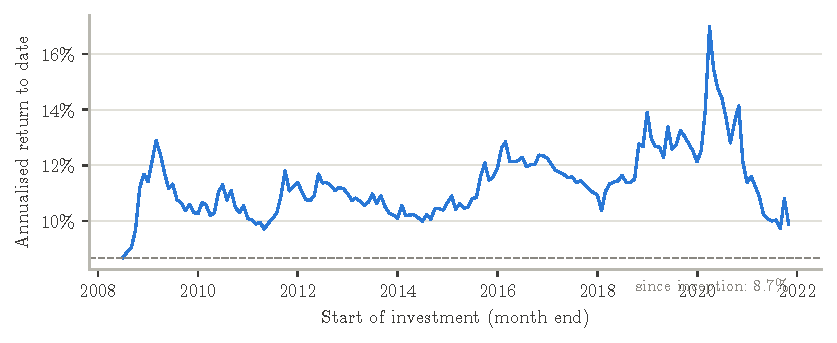
\includegraphics[width=\linewidth]{start_date.pdf}
\caption{Annualised total return from each month end to the latest close (starting points with at least five years of history).}
\end{figure}
Because VT was launched just before the 2008 crash, ``since inception'' figures are among the least favourable available. Starting at any year end between 2008 and 2021 would have delivered between 9.9\% (2021) and 13.9\% (2018) a year to date, against 8.7\% since inception. Performance statistics should always be read together with their start and end dates.

\keep{16}\subsection{The cost of missing the best days}
\begin{figure}[H]
\centering
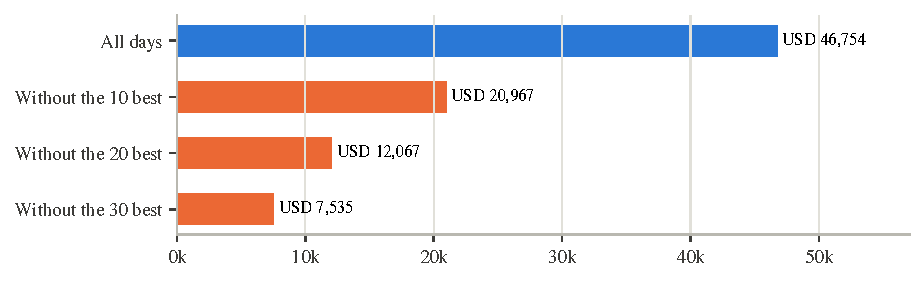
\includegraphics[width=\linewidth]{best_days.pdf}
\caption{Final value of USD 10{,}000 invested at inception, with and without the best trading days.}
\end{figure}
Missing the 10 best days out of 4,615 cuts the annualised return from 8.7\% to 4.0\%. The reverse exercise is just as striking: avoiding the 10 worst days would have lifted the final value to USD 112,534. 7 of the 10 best days fall within two weeks of one of the 10 worst. They occur in the same crisis periods: avoiding the worst days without missing the best would require perfect timing.

\keep{16}\subsection{Monthly savings plan and lump-sum investing}
\begin{figure}[H]
\centering
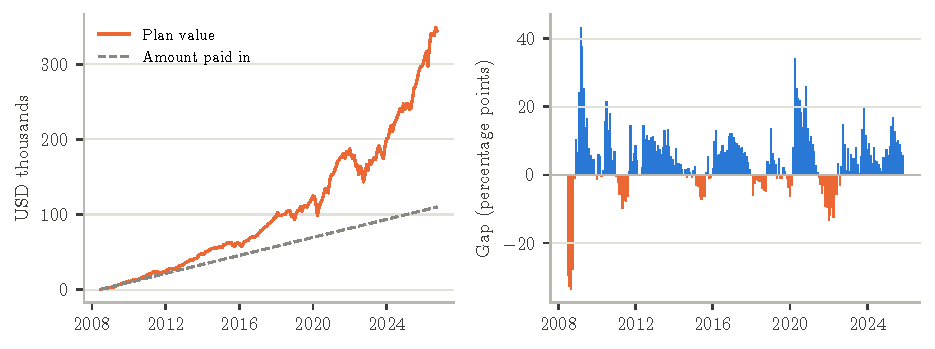
\includegraphics[width=\linewidth]{savings.pdf}
\caption{Left: value of a USD 500 monthly plan vs amount paid in. Right: lump sum minus 12-month averaging, value gap after 12 months, by starting month.}
\end{figure}
Investing USD 500 at the end of every month since inception (220 contributions, USD 110,000 in total) would be worth USD 338,740 today, an internal rate of return of 11.1\% a year, above the 8.7\% of a single investment at inception because most of the money was invested after the 2008--2009 crash.

Across the 209 possible monthly starting points, investing a sum all at once beat spreading it over 12 months (with the uninvested cash earning the T-bill rate) in 72\% of cases, with an average advantage of 4.5\% after 12 months. Because the market rises most of the time, waiting costs money on average; averaging in mainly limits the regret of investing just before a decline. The starting points overlap, so this frequency is descriptive rather than a precise probability.

% ---------------------------------------------------------------- 5
\keep{24}
\section{A Swiss investor's perspective}
\begin{figure}[H]
\centering
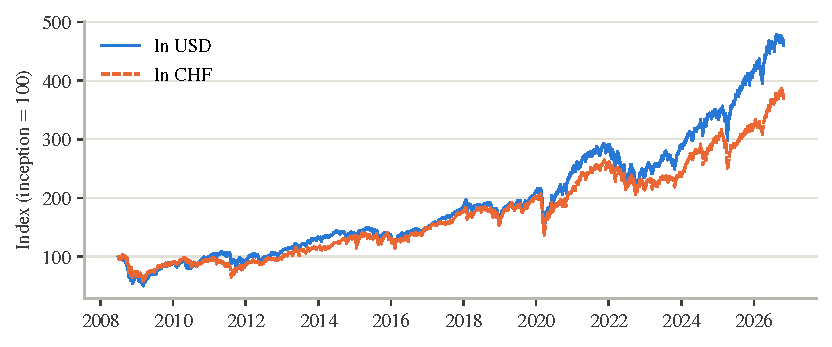
\includegraphics[width=\linewidth]{chf.pdf}
\caption{Total return in USD and in CHF, rebased to 100 at inception.}
\end{figure}

\begin{table}[H]
\small
\caption{VT in US dollars and in Swiss francs.}
\begin{tabularx}{\linewidth}{L r r}
\toprule
 & \textbf{In USD} & \textbf{In CHF} \\
\midrule
Annualised total return & 8.7\% & 7.4\% \\
Annualised volatility (monthly returns) & 16.5\% & 14.9\% \\
USD/CHF over the period & -- & 1.0237 $\rightarrow$ 0.8249 ($-$1.2\% a year) \\
Correlation of VT with USD/CHF (weekly / daily) & -- & $-$0.24 / $-$0.05 \\
\bottomrule
\end{tabularx}
\end{table}
The dollar depreciated against the franc, costing an unhedged Swiss investor about 1.3\% of return a year. The weekly correlation between VT and USD/CHF is $-$0.24; the daily correlation, $-$0.05, is biased towards zero because Yahoo's daily currency and ETF closes are taken at different times of day. The dollar tends to strengthen against the franc when equities fall, which cushions part of the losses in CHF. Because VT is a global fund, its true exposure is to a basket of currencies: USD/CHF captures only part of the currency effect. All figures are before Swiss income tax and the 15\% US withholding tax on dividends, which a Swiss resident can usually credit against Swiss tax.

% ---------------------------------------------------------------- 6
\keep{24}
\section{Data validation}
\begin{table}[H]
\small
\caption{Total returns from Yahoo adjusted prices vs Vanguard's published returns, to 30 September 2026.}
\begin{tabularx}{\linewidth}{L r r r r}
\toprule
\textbf{Period} & \textbf{Vanguard, market price} & \textbf{This report} & \textbf{Gap (pp)} & \textbf{Vanguard, NAV} \\
\midrule
Third quarter 2026 & 0.83\% & 0.83\% & +0.00 & 0.76\% \\
Year to date & 12.86\% & 12.86\% & $-$0.00 & 12.83\% \\
1 year & 16.45\% & 16.45\% & +0.00 & 16.32\% \\
3 years & 21.46\% & 21.45\% & $-$0.01 & 21.42\% \\
5 years & 11.36\% & 11.35\% & $-$0.01 & 11.34\% \\
10 years & 12.32\% & 12.32\% & $-$0.00 & 12.32\% \\
Since inception & 8.78\% & 8.81\% & +0.03 & 8.78\% \\
\bottomrule
\end{tabularx}
\end{table}
\note{Periods of one year or more are annualised. Source: Vanguard fact sheet F3141 (data as of 30 September 2026), stored in \texttt{data/reference/}.}

Yahoo's adjusted prices are not an official source, so the total returns used in this report were checked against the market-price returns published by Vanguard. For all standard periods the two agree to within 0.01 percentage point. The small gap since inception arises because Vanguard measures from the launch on 24 June 2008, two trading days before the first Yahoo closing price. The ETF's market price and its net asset value (NAV) also track each other closely.

% ---------------------------------------------------------------- 7
\keep{20}
\section{Limitations}
\begin{itemize}[leftmargin=1.2em,itemsep=0.3em,topsep=0.2em]
  \item \textbf{One asset, one period.} All results come from a single fund over eighteen years that include one global financial crisis, one pandemic crash and a long bull market. Estimates of mean returns and Sharpe ratios are imprecise over such horizons, as the confidence intervals show.
  \item \textbf{Start date.} VT was launched just before the 2008 crash, which depresses every ``since inception'' figure and works against timing rules that would have protected investors during that crash.
  \item \textbf{Data source.} Yahoo Finance is not an official source, and its adjusted prices can be revised retroactively. The validation against Vanguard covers a single reference date.
  \item \textbf{Market price vs NAV.} The analysis uses closing market prices. The daily autocorrelation may partly reflect gaps between the market price and the net asset value, which cannot be tested without daily NAV data.
  \item \textbf{Taxes and costs.} Returns are gross of investor-level taxes and trading costs (fund expenses are already reflected in the price). Dividends are assumed to be reinvested at the closing price on the ex-dividend date.
  \item \textbf{Model choices.} GARCH(1,1) with symmetric Student-$t$ errors does not capture the asymmetric response of volatility to losses (leverage effect) nor the skewness of large losses. Bootstrap results assume that the dependence structure of the past repeats.
\end{itemize}

% ---------------------------------------------------------------- 8
\keep{12}
\section{Conclusion}
The evidence describes a broadly diversified equity fund that has delivered the equity risk premium with the usual features of equity returns: fat tails, volatility that clusters and persists, and deep but temporary drawdowns. Prices are close to a random walk at the horizons that matter to investors; the one statistically robust anomaly, a small negative daily autocorrelation, is too small and too concentrated in crises to be exploited, and simple timing rules or calendar strategies did not add value. For long-term investors, the main lessons are about horizon and discipline rather than prediction: the probability of loss falls with the holding period but never reaches zero, and missing a handful of days in the middle of a crisis is as costly as suffering the worst of it.

\section*{Data, methods and reproducibility}
\note{Source: Yahoo Finance, downloaded with the \texttt{yfinance} library and updated automatically (GitHub repository \url{https://github.com/cedricmasset98/donnees-marche}). VT: daily closing prices and prices adjusted for dividends and splits (``Adj Close''). Risk-free rate: 13-week US T-bill (\texttt{\^{}IRX}). Currency: USD/CHF (\texttt{CHF=X}). Annualised returns use calendar time; annualised volatility, Sharpe and Sortino ratios use monthly returns; Sharpe confidence intervals follow \citet{mertens2002} and \citet{opdyke2007}, allowing for skewness and kurtosis. Bootstrap results use the fixed seed 20080626. Data file fingerprint (SHA-256 of \texttt{data/VT.csv}): \texttt{bfdcdac71dc770d2}. Software: Python 3.13.17, pandas 3.0.5, NumPy 2.5.3, SciPy 1.18.1, Matplotlib 3.11.2. These analyses are descriptive and historical; they do not constitute investment advice.}

\begin{thebibliography}{9}
\footnotesize
\setlength{\itemsep}{0.2em}
\bibitem[Bollerslev(1986)]{bollerslev1986}
Bollerslev, T. (1986). Generalized autoregressive conditional heteroskedasticity. \emph{Journal of Econometrics}, 31(3), 307--327.
\bibitem[Christoffersen(1998)]{christoffersen1998}
Christoffersen, P.~F. (1998). Evaluating interval forecasts. \emph{International Economic Review}, 39(4), 841--862.
\bibitem[Holm(1979)]{holm1979}
Holm, S. (1979). A simple sequentially rejective multiple test procedure. \emph{Scandinavian Journal of Statistics}, 6(2), 65--70.
\bibitem[Kupiec(1995)]{kupiec1995}
Kupiec, P.~H. (1995). Techniques for verifying the accuracy of risk measurement models. \emph{Journal of Derivatives}, 3(2), 73--84.
\bibitem[Lo and MacKinlay(1988)]{lo1988}
Lo, A.~W. and MacKinlay, A.~C. (1988). Stock market prices do not follow random walks: Evidence from a simple specification test. \emph{Review of Financial Studies}, 1(1), 41--66.
\bibitem[Mertens(2002)]{mertens2002}
Mertens, E. (2002). Comments on variance of the IID estimator in Lo (2002). Working paper, University of Basel.
\bibitem[Opdyke(2007)]{opdyke2007}
Opdyke, J.~D. (2007). Comparing Sharpe ratios: So where are the p-values? \emph{Journal of Asset Management}, 8(5), 308--336.
\bibitem[Politis and Romano(1994)]{politis1994}
Politis, D.~N. and Romano, J.~P. (1994). The stationary bootstrap. \emph{Journal of the American Statistical Association}, 89(428), 1303--1313.
\end{thebibliography}

\end{document}